%%%%%%%%%%%%%%%%%%%%%%%%%%%%%%%%%%%%%%%%%%%%%%%%%%%%%%%%%%%%%%%%%%%%%%%%%%%
%% This file is part of the book
%%
%% Algorithmic Graph Theory
%% http://code.google.com/p/graph-theory-algorithms-book/
%%
%% Copyright (C) 2009, 2010 Minh Van Nguyen <nguyenminh2@gmail.com>
%%
%% See the file COPYING for copying conditions.
%%%%%%%%%%%%%%%%%%%%%%%%%%%%%%%%%%%%%%%%%%%%%%%%%%%%%%%%%%%%%%%%%%%%%%%%%%%

\subfigure[]{
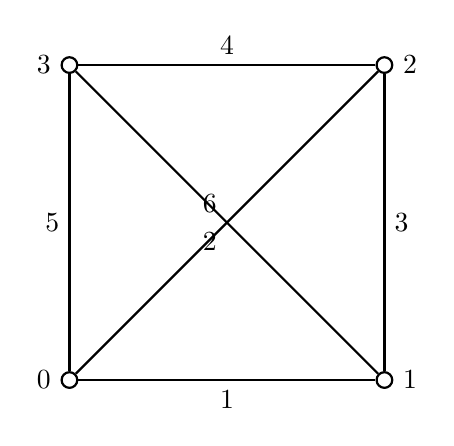
\begin{tikzpicture}
[nodedecorate/.style={shape=circle,inner sep=2pt,draw,thick},%
  linedecorate/.style={-,thick}]
% nodes or vertices
\node (0) at (0,0) [nodedecorate] {};
\node [left] at (0.west) {$0$};
\node (1) at (4,0) [nodedecorate] {};
\node [right] at (1.east) {$1$};
\node (2) at (4,4) [nodedecorate] {};
\node [right] at (2.east) {$2$};
\node (3) at (0,4) [nodedecorate] {};
\node [left] at (3.west) {$3$};
% edges or lines
\path
(0) edge[linedecorate] node[below]{$1$} (1)
(0) edge[linedecorate] node[below left] {$2$} (2)
(0) edge[linedecorate] node[left]{$5$} (3)
(1) edge[linedecorate] node[right]{$3$} (2)
(1) edge[linedecorate] node[above left] {$6$} (3)
(2) edge[linedecorate] node[above]{$4$} (3);
\end{tikzpicture}
}
\qquad
\subfigure[]{
\begin{tikzpicture}
[nodedecorate/.style={shape=circle,inner sep=2pt,draw,thick},%
  linedecorate/.style={-,thick}]
% nodes or vertices
\node (3) at (0,0) [nodedecorate] {};
\node [right] at (3.east) {$3$};
\node (2) at (1,2) [nodedecorate] {};
\node [right] at (2.east) {$2$};
\node (0) at (2,4) [nodedecorate] {};
\node [right] at (0.east) {$0$};
\node (1) at (3,6) [nodedecorate] {};
\node [right] at (1.east) {$1$};
% edges or lines
\path
(3) edge[linedecorate] node[left]{$4$} (2)
(2) edge[linedecorate] node[left]{$2$} (0)
(0) edge[linedecorate] node[left]{$1$} (1);
\end{tikzpicture}
}
